
\chapter{Test scenes}
\label{ch:test_scenes}

For testing the surface reconstruction algorithms discussed in the preceding chapters, a few test scenes are proposed.
The test scenes and their configurations are shown in \cref{tbl:test_scenes}.
%
\begin{table}[h]
	\centering
	\begin{tabular}{lrrrrrrrr}
		Scene          & SVs  & cells & surf. & tri.  & s\textsubscript{max} & s\textsubscript{avg} \\
		\midrule
		\cubes          &    1 & \SI{  1}{\kilo\nothing} & \SI{47}{\percent} & \SI{  0.8}{\kilo\nothing} &  2 & 1.1 \\
		\cylindersd   &    1 & \SI{  1}{\kilo\nothing} & \SI{22}{\percent} & \SI{    7}{\kilo\nothing} &  2 & 1.1 \\
		\cylinders      &    1 & \SI{  1}{\kilo\nothing} & \SI{22}{\percent} & \SI{    4}{\kilo\nothing} &  2 & 1.1 \\
		\cylinderhead &   20 & \SI{ 75}{\kilo\nothing} & \SI{21}{\percent} & \SI{   80}{\kilo\nothing} &  3 & 1.2 \\
		\impeller       & 2383 & \SI{400}{\kilo\nothing} & \SI{16}{\percent} & \SI{ 6000}{\kilo\nothing} & 64 & 5.5 \\
		\impellerhalf    & 1191 & \SI{400}{\kilo\nothing} & \SI{13}{\percent} & \SI{ 3000}{\kilo\nothing} & 64 & 3.6 \\
		\turbine        &  480 & \SI{200}{\kilo\nothing} & \SI{17}{\percent} & \SI{16000}{\kilo\nothing} &  6 & 2.3 \\
	\end{tabular}
	\caption[Test scenes]{
		The selected test scenes with their major parameters.
		These are the name of a scene, the number of swept volumes, the total number of cells of the regular grid, the amount of surface cells in the grid, \ie cells which have to be processed, the total amount of triangles in the grid as well as the maximum and average amount of structures in a cell.
	}
	\label{tbl:test_scenes}
\end{table}

The \cubes scene is a simple intersection between a cubic stock and a cuboid swept volume.
It is also used as an example in the discussion of the concept of the direct intersection approach at the beginning of this chapter in \cref{fig:cube2}.
Instead of no grid, a small one with a resolution of $10\times10\times10$ cells is used.
This scene is used as a proof of concept for each surface reconstruction algorithm in this thesis.

The \cylinders and \cylindersd scenes each consist of a broader cylindrical stock with a smaller cylindrical swept volume drilled out.
The cylinders in the \cylindersd scene are triangulated into smaller and more regular triangles by constraining the edge lengths of the output triangles.
The cylinders in the \cylinders scene contain longer and thinner triangles.
The \cylindersd scene requires more triangles to approximate the cylinders.
Both scenes also use the same small grid resolution as the \cubes scene.
These two scenes should have an almost identical visual outcome but quite different stress on the numeric robustness of the extraction.

The \cylinderhead scene was the initial test scene when the raycasting subsystem was developed, \cf \cref{ch:previous_work}.
It is the smallest and easiest of the practical scenes used for benchmarking.
The \cylinderhead uses a medium sized grid of $50\times50\times30$ cells with a moderate, but still little, number of triangles and swept volumes.

The \impeller scene provides a good real world example of a typical machining scenario.
It contains a few thousand swept volumes organized in a larger grid of $100\times100\times40$ cells.
With 6 million stored triangles and a lot more structures in each cell, the \impeller scene should already pose a serious workload for the tested algorithms.
To analyze the effect of the number of swept volumes, a second version of the \impeller scene has been created, the \impellerhalf scene, where only half the number of swept volumes have been loaded.

Finally, the \turbine scene depicts a further practical example.
The scene is conceived to stress the swept volume computation by its complex cutting tool, a fir-tree cutter.
The fine tessellation of the cutter mesh results in high resolution swept volumes and the largest amount of triangles stored in a test scene.

The amount of triangles in each grid cell varies greatly between the test scenes and also in the scenes themselves.
This property is interesting, as it has the largest impact on algorithms which have to iterate over the triangles of a cell.
Furthermore, largely divergent triangle counts inside cells challenge schedulers in parallel processing of cells and increase branch divergence on GPU architectures.
An optimal distribution would be an almost empty histogram with a peak at a certain location, meaning all surface cells contain roughly the same number of triangles.
\Cref{fig:histograms} shows histograms of the triangles per cell distribution for the test scenes of \cref{tbl:test_scenes}.
%
\begin{figure}[!]
	\centering
	\begin{subfigure}[b]{0.49\textwidth}
		\centering
		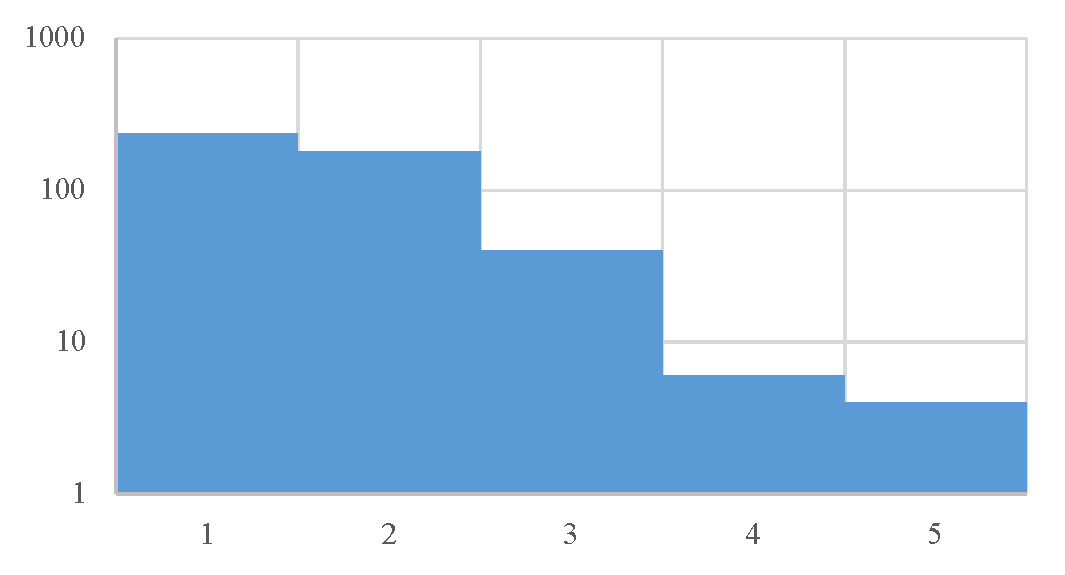
\includegraphics[width=\textwidth]{c_hist}
		\caption{\cubes}
		\label{fig:cube2_histogram}
	\end{subfigure}
	\begin{subfigure}[b]{0.49\textwidth}
		\centering
		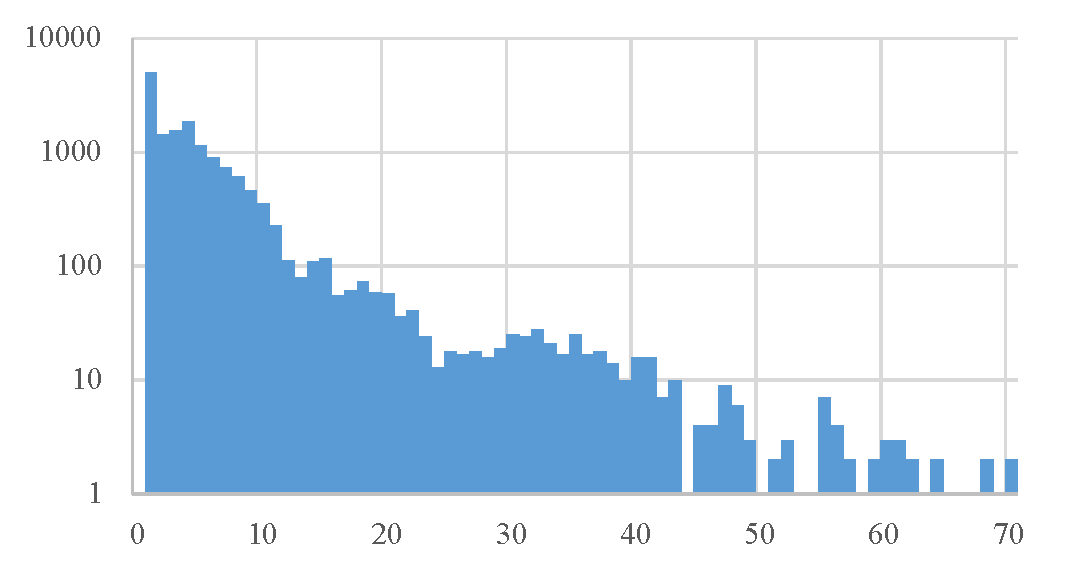
\includegraphics[width=\textwidth]{ch_hist}
		\caption{\cylinderhead}
		\label{fig:cylinder_head_histogram}
	\end{subfigure}
	\begin{subfigure}[b]{0.49\textwidth}
		\centering
		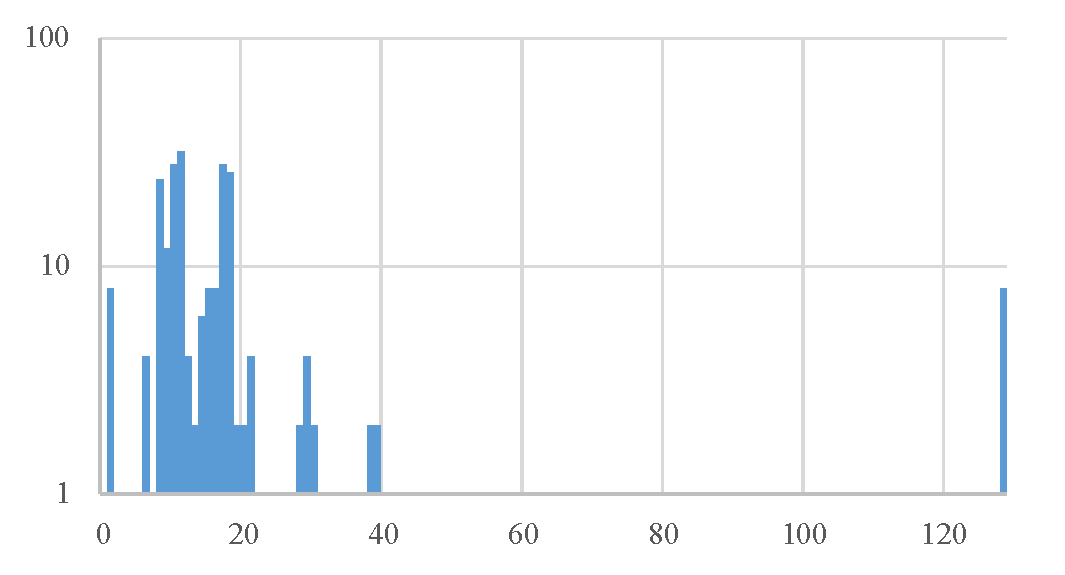
\includegraphics[width=\textwidth]{cy_hist}
		\caption{\cylinders}
		\label{fig:cylinders_histogram}
	\end{subfigure}
	\begin{subfigure}[b]{0.49\textwidth}
		\centering
		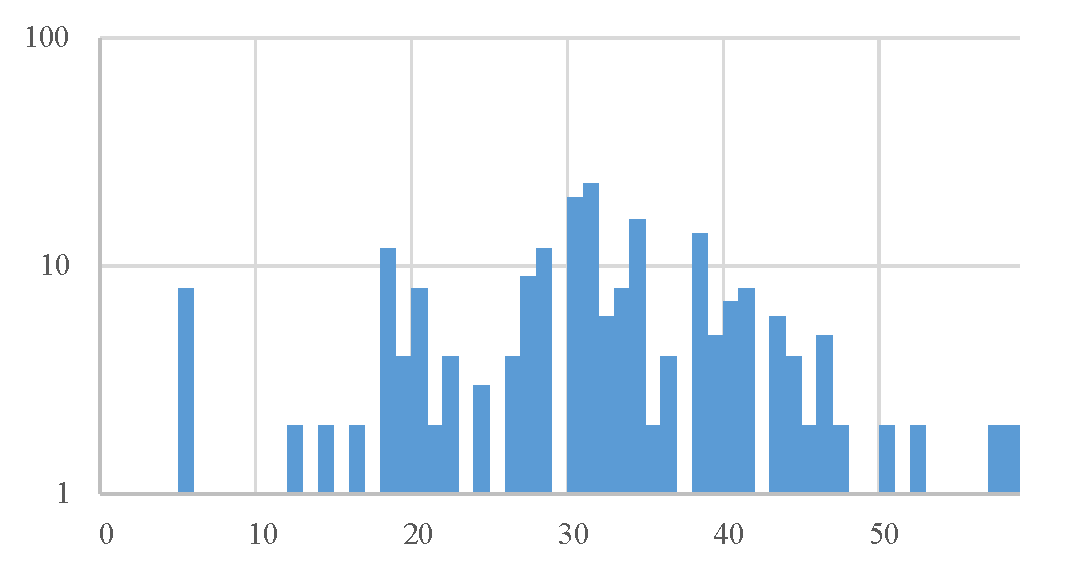
\includegraphics[width=\textwidth]{cyd_hist}
		\caption{\cylindersd}
		\label{fig:cylinders_d_histogram}
	\end{subfigure}
	\begin{subfigure}[b]{0.49\textwidth}
		\centering
		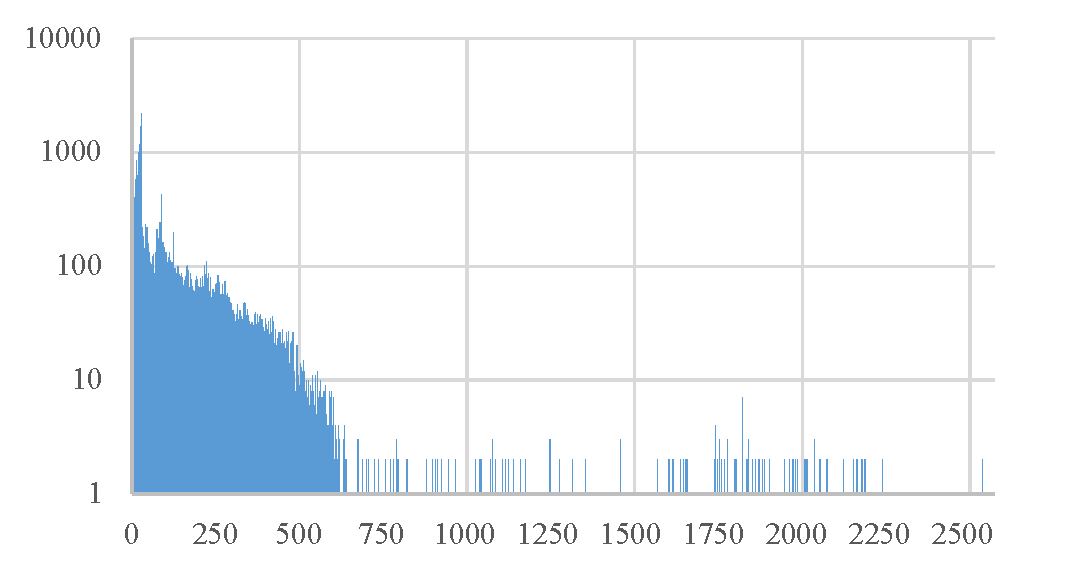
\includegraphics[width=\textwidth]{hq_hist}
		\caption{\impeller}
		\label{fig:impeller_histogram}
	\end{subfigure}
	\begin{subfigure}[b]{0.49\textwidth}
		\centering
		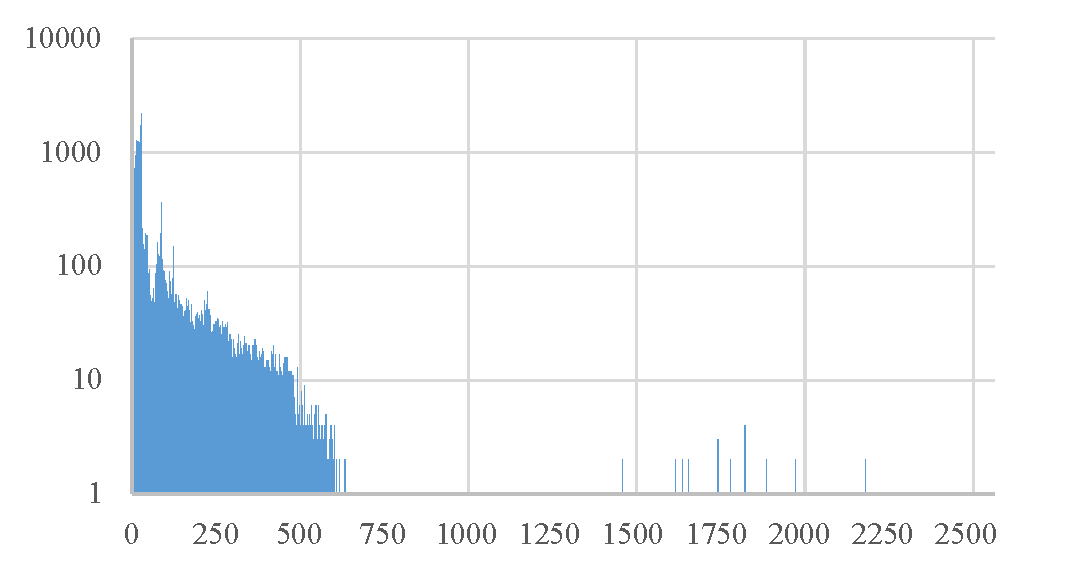
\includegraphics[width=\textwidth]{hq2_hist}
		\caption{\impellerhalf}
		\label{fig:impeller_2_histogram}
	\end{subfigure}
	\begin{subfigure}[b]{0.49\textwidth}
		\centering
		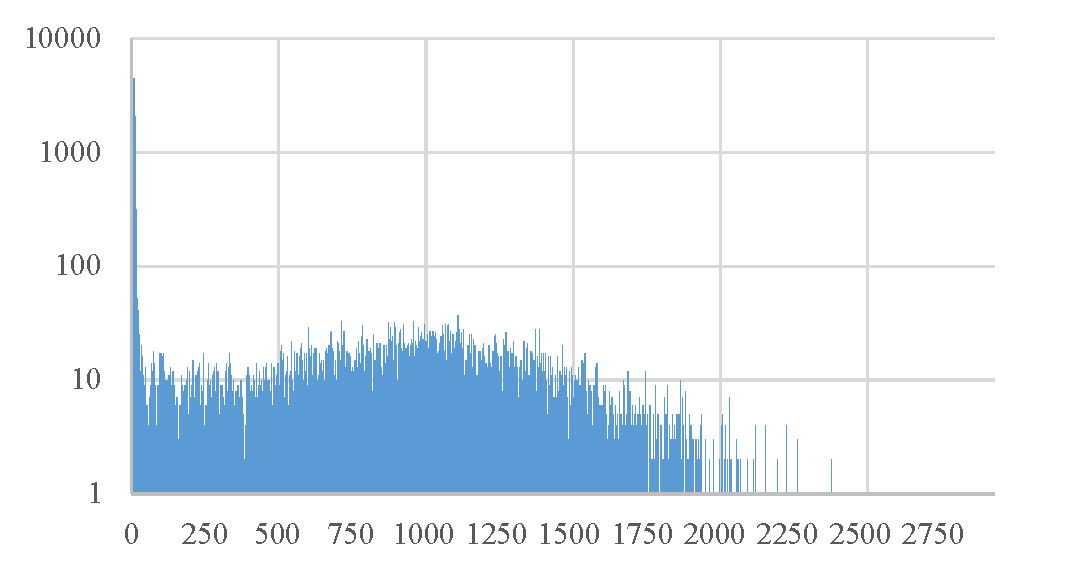
\includegraphics[width=\textwidth]{tr_hist}
		\caption{\turbine}
		\label{fig:turbine_histogram}
	\end{subfigure}
	\caption[Test scene histograms]{
		Histograms showing the distribution of triangle counts per cell for the selected test scenes in \cref{tbl:test_scenes}.
		The horizontal axis shows the number of triangles per cell.
		The vertical axis is logarithmic and shows the number of cells with a specific triangle count.
	}
	\label{fig:histograms}
\end{figure}

The \cubes scene contains few triangles in general.
Most cells contain only one or two triangles and probably not more than one structure.
Larger cells contain four or five triangles occur infrequent.
In general, the distribution is quite compact.

The \cylinderhead is characterized by a quite divergent distribution, although the range is still modest from many cells with a small triangle count to only a few cells with 40 to 70 triangles.

Considering the cylindrical scenes, the histograms show the difference in the total number of triangles.
As the \cylindersd scene contains more, smaller and more regular triangles, its cells are also occupied by more triangles.
Whereas the \cylinders scene holds mostly between 5 and 20 triangles, the cells of the \cylindersd scene contain mostly between 20 and 45 triangles.
Nevertheless, despite their lower triangle counts, there is a peek of triangles in the \cylinders scene at 128 triangles, which are cells at the center of the cylinder.

The \impeller scene shows a quite good but broad distribution with most cells containing between 1 and 100 triangles.
The further large part of all cells store between 100 and around 500 triangles.
Unfortunately, the \impeller scene contains several cells with extraordinary high quantities of triangles, up to 2574 triangles in a single cell, 2563 for the \impellerhalf scene.

Finally, the \turbine scene attracts attention by its smooth distribution of triangle counts.
Despite its uniformity, such distributions are unfortunately rather disadvantages as the workload per cell is highly diverse.
Furthermore, the triangle counts per cell are quite high with amounts of up to 2000 triangles per cell occurring quite often.
Cells with even more triangles exist only marginally.

For visual reference, \cref{fig:raycasted_scenes} shows images of the selected test scenes raycasted using the VML.
%
\begin{figure}[!]
	\centering
	\begin{subfigure}[b]{0.43\textwidth}
		\centering
		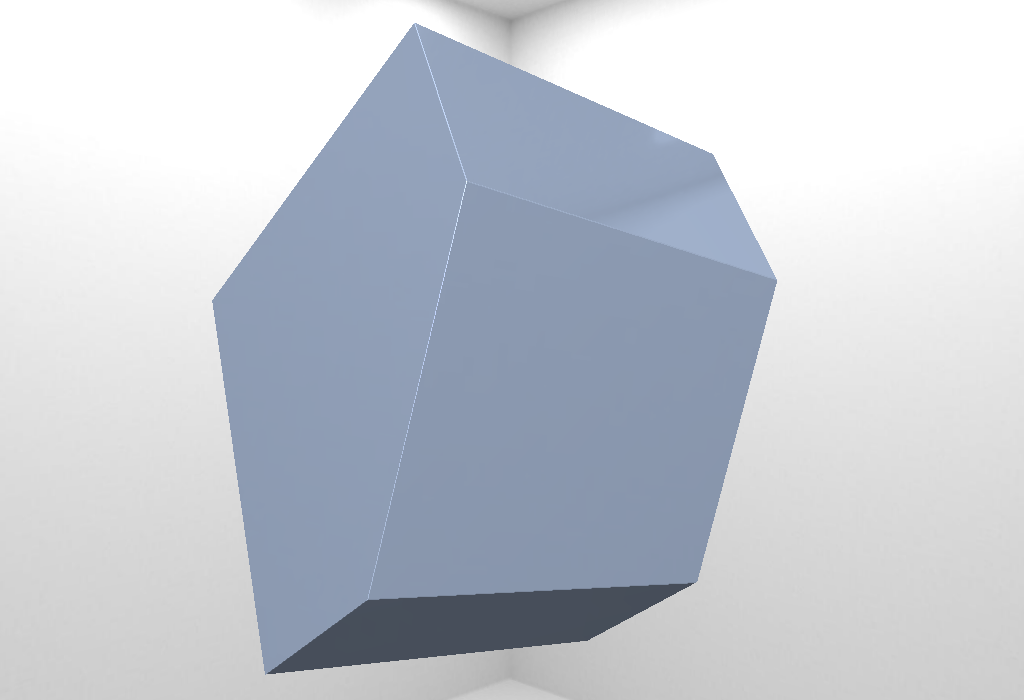
\includegraphics[width=\textwidth]{raycasted_cube2}
		\caption{\cubes}
		\label{fig:cube2_raycasted}
	\end{subfigure}
	\begin{subfigure}[b]{0.43\textwidth}
		\centering
		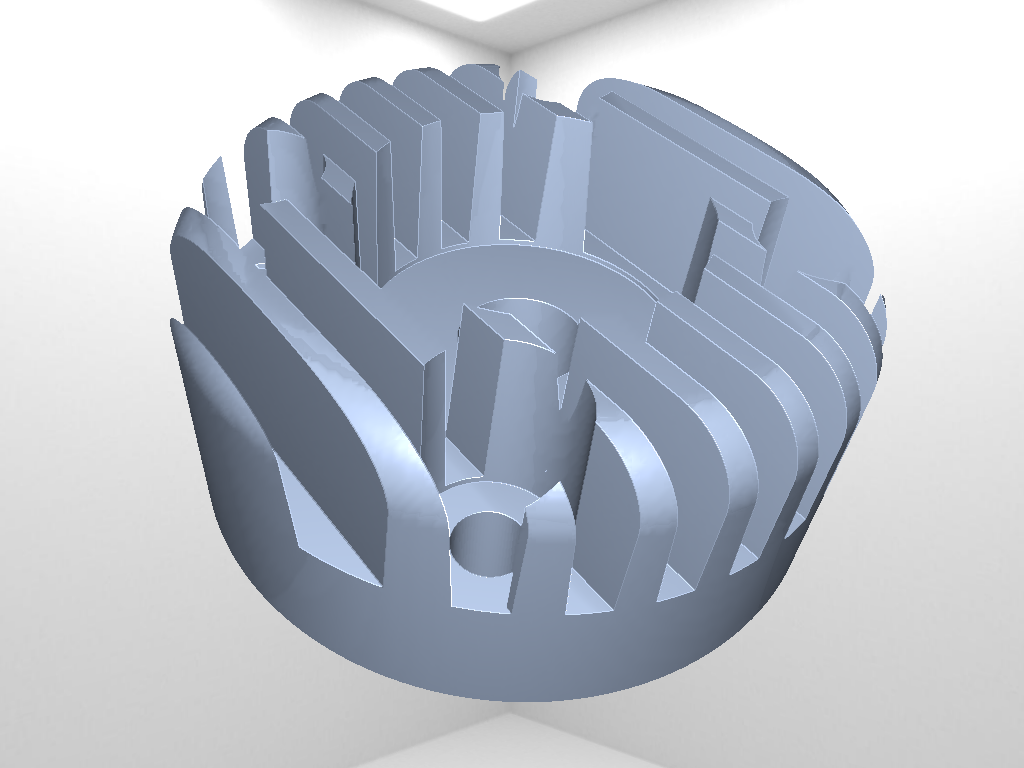
\includegraphics[width=\textwidth]{raycasted_cylinder_head}
		\caption{\cylinderhead}
		\label{fig:cylinder_head_raycasted}
	\end{subfigure}
	\begin{subfigure}[b]{0.43\textwidth}
		\centering
		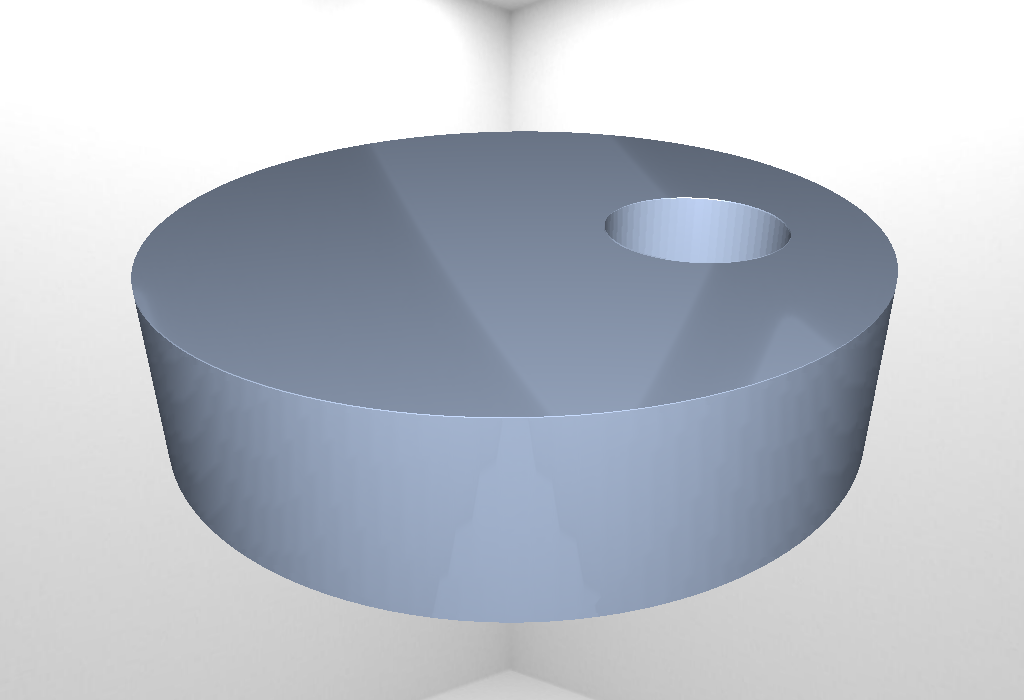
\includegraphics[width=\textwidth]{raycasted_cylinders}
		\caption{\cylinders}
		\label{fig:cylinders_raycasted}
	\end{subfigure}
	\begin{subfigure}[b]{0.43\textwidth}
		\centering
		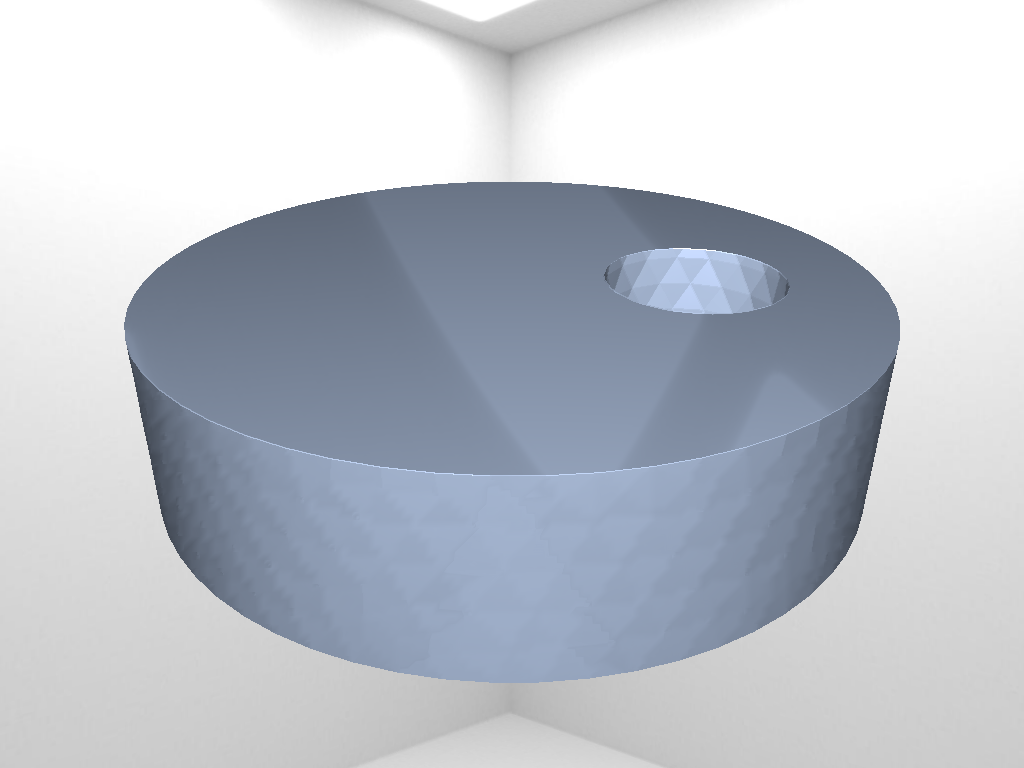
\includegraphics[width=\textwidth]{raycasted_cylinders_d}
		\caption{\cylindersd}
		\label{fig:cylinders_d_raycasted}
	\end{subfigure}
	\begin{subfigure}[b]{0.43\textwidth}
		\centering
		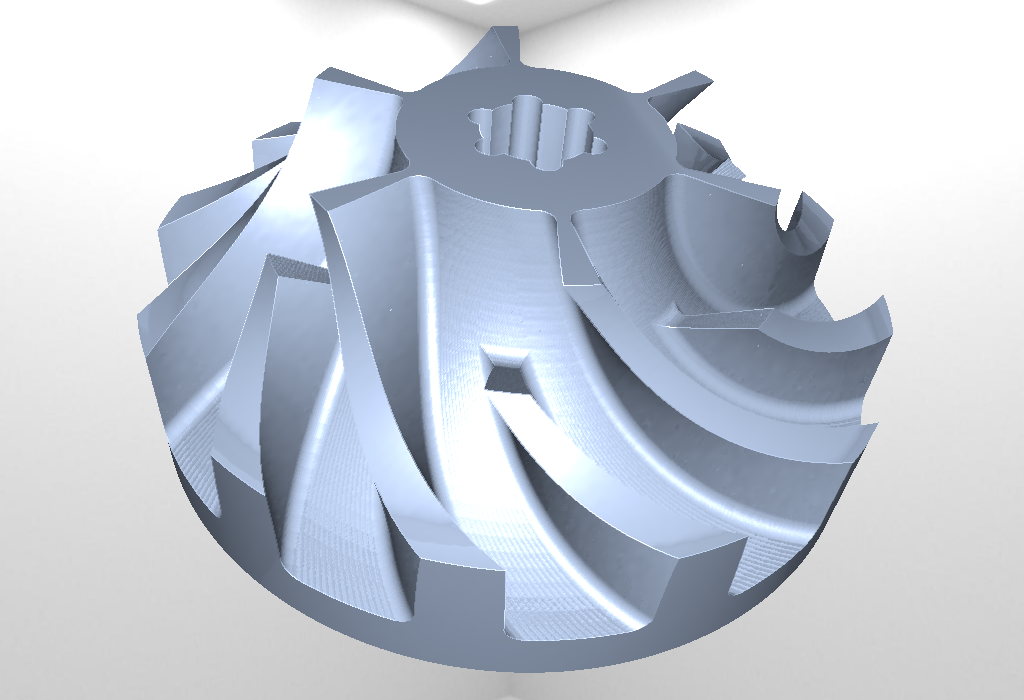
\includegraphics[width=\textwidth]{raycasted_impeller}
		\caption{\impeller}
		\label{fig:impeller_raycasted}
	\end{subfigure}
	\begin{subfigure}[b]{0.43\textwidth}
		\centering
		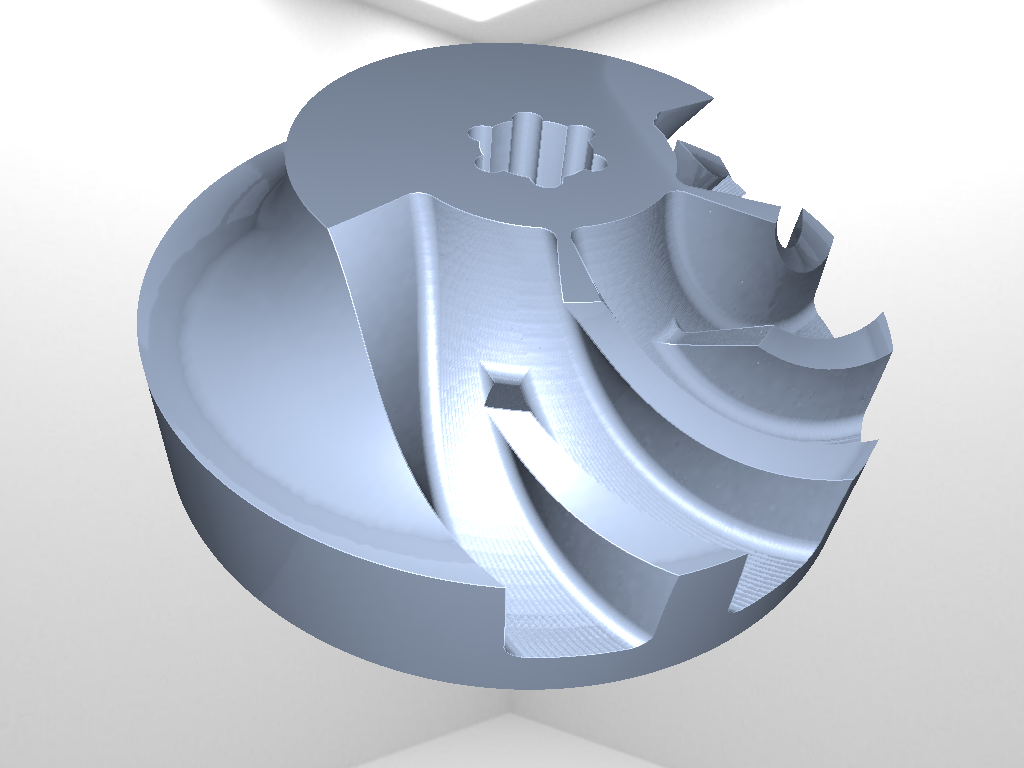
\includegraphics[width=\textwidth]{raycasted_impeller_2}
		\caption{\impellerhalf}
		\label{fig:impeller_2_raycasted}
	\end{subfigure}
	\begin{subfigure}[b]{0.43\textwidth}
		\centering
		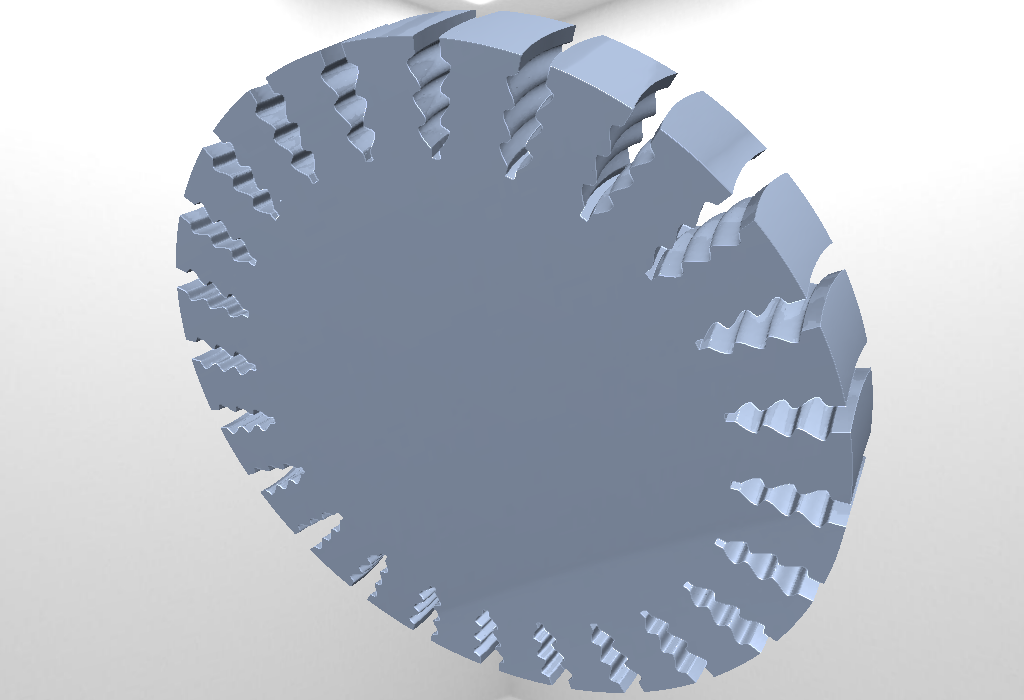
\includegraphics[width=\textwidth]{raycasted_turbine}
		\caption{\turbine}
		\label{fig:turbine_raycasted}
	\end{subfigure}
	\caption[Raycasted images of test scenes]{
		Images of the test scenes given in \cref{tbl:test_scenes}.
		The images are created by the raycasting system of the VML in combination with visual enhancements using OpenGL shaders.
		These images are used as references for the renderings of result meshes produced by the extraction methods discussed in this thesis.
	}
	\label{fig:raycasted_scenes}
\end{figure}
